Un parametro utile ad indicare quanto un dispositivo MOSFET possa regolare la corrente di drain $I_D$, attraverso la tensione $V_{GS}$, è la transconduttanza $g_m$. essa è definita dal rapporto incrementale:

$$g_m = \frac{\partial I_D}{\partial V_{GS}}$$

Nel caso di $I_D-V_{GS}$ in regione lineare, si ottiene l'espressione:

$$g_m = \frac{W}{L} \cdot \mu \cdot C_{ox} \cdot (V_{GS} - V_{th})$$


\subsection{Calcolo della transconduttanza}
Derivare dei dati discontinui porta sempre, o quasi sempre, ad avere delle curve spezzate, per le quali è difficile trarre informazioni utili.
Questo è stato il caso per la transconduttanza; la figura \ref{fig:gm_smooth:no_smooth} (curva di sinistra) rappresenta la $g_m$ di un transistor  MOSFET a canale N, con $ W = 100\mu m$ e $L = 30 nm$ senza eseguire nessun tipo di smooth; in particolare, per alte $V_{GS}$, il difetto è molto marcato. Per ridurre questo effetto, oltre ad applicare alla fine uno smooth di ampiezza $5$, due valori prima e due valori dopo; abbiamo calcolato due transconduttanze, la prima ${g_m}^{\prime}$ normalmente, mentre, la seconda ${g_m}^{\prime \prime}$ abbiamo eseguito il rapporto incrementale tra $I_D$ e ${V_{GS}}^*$, tensione gate-source shiftata di una posizione, duplicando il primo valore ed eliminando l'ultimo. In seguito abbiamo trovato la transconduttanza come la media dei singoli valori: 
$${g_m}_i = \frac{{g_m}_i^{\prime} + {g_m}_i^{\prime \prime}}{2} \text{ } i \in [1 , 2 , 3 . . .]$$

Trovando, per il dispositivo in questione, la curva a figura \ref{fig:gm_smooth:smooth}(curva a destra).

\begin{figure}[t]
    \centering
    % W = 100 
    \subfloat[$g_m$ senza utilizzo dello smooth]{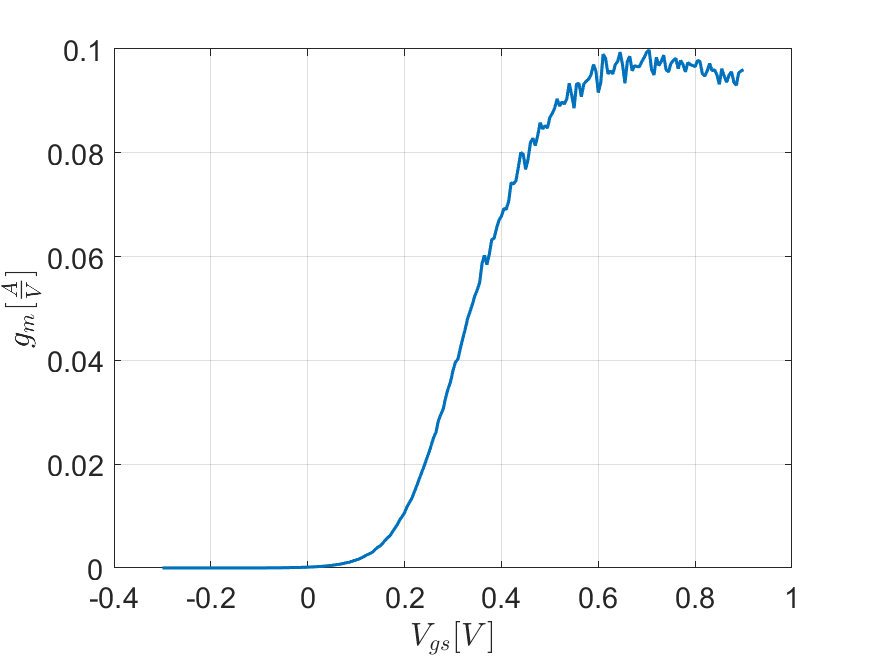
\includegraphics[width=0.49\textwidth]{./capitolo2/transconduttanza/estrazione_dati/gm_no_smooth.png}\label{fig:gm_smooth:no_smooth}}
    \subfloat[$g_m$ con utilizzo di smooth]{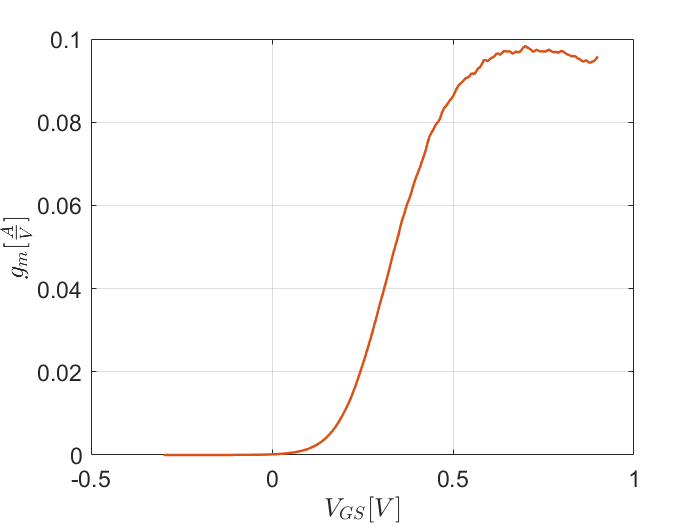
\includegraphics[width=0.49\textwidth]{./capitolo2/transconduttanza/estrazione_dati/gm_smooth.png}\label{fig:gm_smooth:smooth}}

    \caption[Confronto $g_m$ senza utilizzo di smooth e con utilizzo di smooth]{Confronto delle transconduttanze calcolate senza applicare smooth e con l'utilizzo di smooth.}
    \label{fig:gm_smooth}
\end{figure}


% \todo[inline]{Da aggiungere cose ho scritto troppo poco}
\vspace{0.5cm}

A figura \ref{fig:gm_w} vengono mostrati i grafici relativi alla transconduttanza per i diversi transistori MOSFET, sia a canale N che P. Avendo imposto, sul dispositivo che effettua le misure statiche, il limite di correte di drain a $100mA$(positiva e negativa); per i dispositivi con larghezza $600\mu m$ e con lunghezze inferiori a $60nm$, questo limite viene raggiunto spiegando così il motivo del crollo della $g_m$ per alte $V_{GS}$

\begin{figure}[t]
    \centering
    % W = 100 
    \includegraphics[width=0.49\textwidth]{./capitolo2/transconduttanza/gm/NMOS/gm_w_100_vds_900_mV.png}
    \includegraphics[width=0.49\textwidth]{./capitolo2/transconduttanza/gm/PMOS/gm_w_100_vds_900_mV.png}

    \vspace{0.5cm}
    % W = 200
    \includegraphics[width=0.49\textwidth]{./capitolo2/transconduttanza/gm/NMOS/gm_w_200_vds_900_mV.png}
    \includegraphics[width=0.49\textwidth]{./capitolo2/transconduttanza/gm/PMOS/gm_w_200_vds_900_mV.png}
    % W = 600
    \vspace{0.5cm}

    \includegraphics[width=0.49\textwidth]{./capitolo2/transconduttanza/gm/NMOS/gm_w_600_vds_900_mV.png}
    \includegraphics[width=0.49\textwidth]{./capitolo2/transconduttanza/gm/PMOS/gm_w_600_vds_900_mV.png}

    \caption[Dati $g_m$ estratti pre-irraggiamento]{Transconduttanza calcolata nei dispositivi MOSFET prima di subire la dose di irraggiamento. canale N, a sinistra, e canale P, a destra, i grafici sono raggruppati per larghezza di canale.}
    \label{fig:gm_w}

\end{figure}


\vspace{0.5cm}

Uno dei effetti delle radiazioni ionizzanti è quella di ridurre la mobilità dei portatori di carica $\mu$ all'interno del canale. Osservando  l'espressione della $g_m$ si nota la proporzionalità diretta con la mobilità dei portatori comportando una riduzione della transconduttanza, all'aumentare della dose assorbita. Per confermare questo effetto, si è calcolata la variazione della transconduttanza, in percentuale, all'aumentare della dose assorbita:

$$\Delta {g_m}_{post} {\%} = \frac{{g_m}_{post} - {g_m}_{pre}}{{g_m}_{pre}}\cdot 100$$

Con ${g_m}_{post}$ si intende il massimo valore della transconduttanza per un certo dosaggio, e similmente per ${g_m}_{pre}$, il massimo valore pre-irraggiamento. L'effetto è stato confermato dai dati sperimentali (vedi tabelle \ref{tab:deltaGm_N} e \ref{tab:deltaGm_P} e figura \ref{fig:delta_gm}) ottenuti dai transistori\footnote{La $V_{DS}$ da cui è stata estratta la transconduttanza è di $0.9V$, nel caso di NMOS, mentre per PMOS $-0.9V$.} sotto osservazione in questo lavoro di tesi.

\begin{table}[t]
    \renewcommand{\arraystretch}{1.3}
    \resizebox{\textwidth}{!}{%
        \begin{tabular}{c c c c c c c c c}
            \toprule
            \multirow{2}{*}{Dispositivo} & \multicolumn{8}{c}{$\Delta g_{m}\% [\sfrac{A}{V}] $}                                                                                \\
            \cmidrule{2-9}
                                         & $5Mrad$                                              & $50Mrad$ & $100Mrad$ & $200Mrad$ & $600Mrad$ & $1Grad$ & $3Grad$ & annealing \\
            \midrule
            100-0.030                       & -0.3866                                              & -0.4273  & -0.7731   & -0.7528   & -1.2004   & -2.2787 & -4.0081 & -4.2930   \\
            \hline
            100-0.060                       & -0.2759                                              & -0.6667  & -1.6092   & -1.6092   & -1.8851   & -2.7126 & -4.6207 & -4.2989   \\
            \hline
            100-0.180                      & 1.1011                                               & 1.1567   & -2.7027   & -2.2356   & -2.2356   & -4.1263 & -6.9069 & -7.0181   \\
            \hline
            200-0.030                       & -0.1333                                              & 0.3758   & -0.9939   & -1.2000   & -1.8667   & -2.7273 & -5.0182 & -5.0788   \\
            \hline
            200-0.060                       & 1.3702                                               & 0        & -1.3823   & -1.4915   & -2.0007   & -3.0799 & -4.8139 & -4.9473   \\
            \hline
            200-0.180                      & 0.5282                                               & 0.3815   & -3.3744   & -3.3451   & -4.5775   & -5.4577 & -9.5364 & -9.5070   \\
            \hline
            600-0.060                       & -1.4440                                              & -1.8532  & -4.0193   & -3.4817   & -4.4765   & -5.1023 & -6.1773 & -6.4902   \\
            \hline
            600-0.180                      & 0.8105                                               & 1.0132   & -4.2553   & -4.5086   & -4.8632   & -5.6738 & -8.0041 & -8.7133   \\
            \bottomrule
        \end{tabular}%
        }
    \caption[Dati $\Delta g_m \%$ al variare della dose assorbita, NMOS]{Variazioni della transconduttanza al variare della dose assorbita in un MOSFET a canale N.}
    \label{tab:deltaGm_N}
\end{table}

\begin{table}[t]
    \renewcommand{\arraystretch}{1.3}
    \resizebox{\textwidth}{!}{%
        \begin{tabular}{c c c c c c c c c}
            \toprule
            \multirow{2}{*}{Dispositivo} & \multicolumn{8}{c}{$\Delta g_{m}\% [\sfrac{A}{V}] $}                                                                                    \\
            \cmidrule{2-9}
                                         & $5Mrad$                                              & $50Mrad$   & $100Mrad$ & $200Mrad$ & $600Mrad$ & $1Grad$  & $3Grad$  & annealing \\
            \midrule
            100-0.030                       & -0.1216                                              & -0.9325    & -1.4393   & -1.1555   & -3.0205   & -4.1557  & -11.2508 & -6.4058   \\
            \hline
            100-0.060                       & -0.1578                                              & -0.8343    & -1.3078   & -1.0372   & -3.1342   & -4.3292  & -12.2435 & -6.5614   \\
            \hline
            200-0.030                       & 0.0797                                               & -0.4461    & -0.7328   & 0.1593    & -1.3223   & -1.4338  & -6.2291  & -3.7757   \\
            \hline
            200-0.060                       & 0.1837                                               & -0.4898    & -0.8878   & -0.2908   & -1.8062   & -2.4797  & -8.8321  & -4.4390   \\
            \hline
            200-0.180                      & -0.6345                                              & -1.7766    & -1.2690   & -1.5228   & -3.2995   & -5.0761  & -18.6548 & -11.1675  \\
            \hline
            600-0.030                       & -0.0069                                              & -0.2477    & -0.3647   & 0.1651    & -0.9770   & -0.7362  & -4.9539  & -3.4884   \\
            \hline
            600-0.060                       & 0.0494                                               & -0.0412    & -0.6837   & 0.1565    & -0.9885   & -1.5568  & -7.4876  & -4.3822   \\
            \hline
            600-0.180                      & 0.1198                                               & -0.4790    & -1.1976   & -1.0579   & -3.2335   & -4.3114  & -17.9441 & -8.8423   \\
            \bottomrule
        \end{tabular}%
    }
    \caption[Dati $\Delta g_m \%$ al variare della dose assorbita, PMOS]{Variazioni della transconduttanza al variare della dose assorbita in un MOSFET a canale P.}
    \label{tab:deltaGm_P}
\end{table}

\begin{figure}[ht]
    \centering
    % W = 100 
    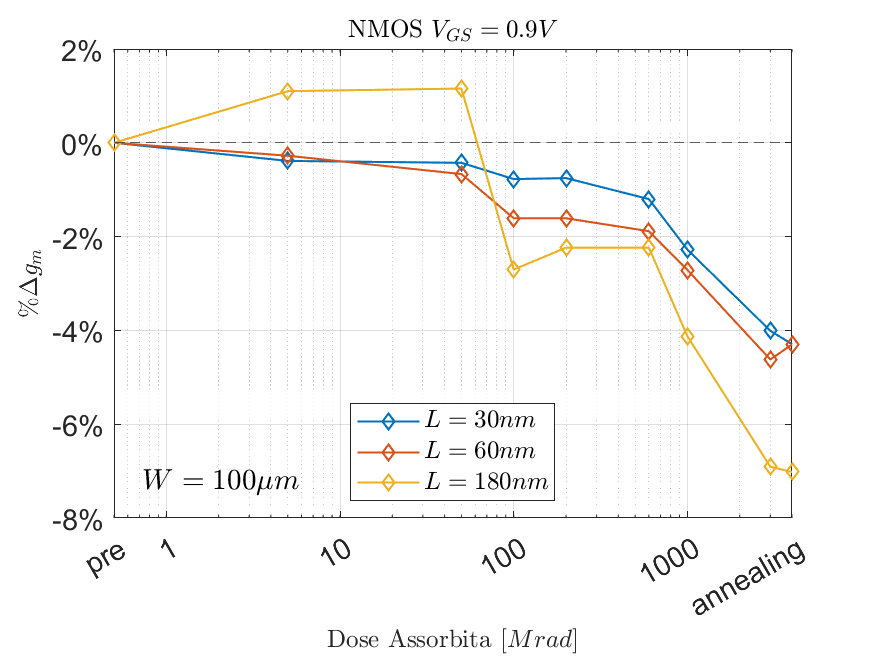
\includegraphics[width=0.49\textwidth]{./capitolo2/transconduttanza/delta_gm_N/vds_0_9/Delta_Gm_NMOS_Vds_0_9_W_100.png}
    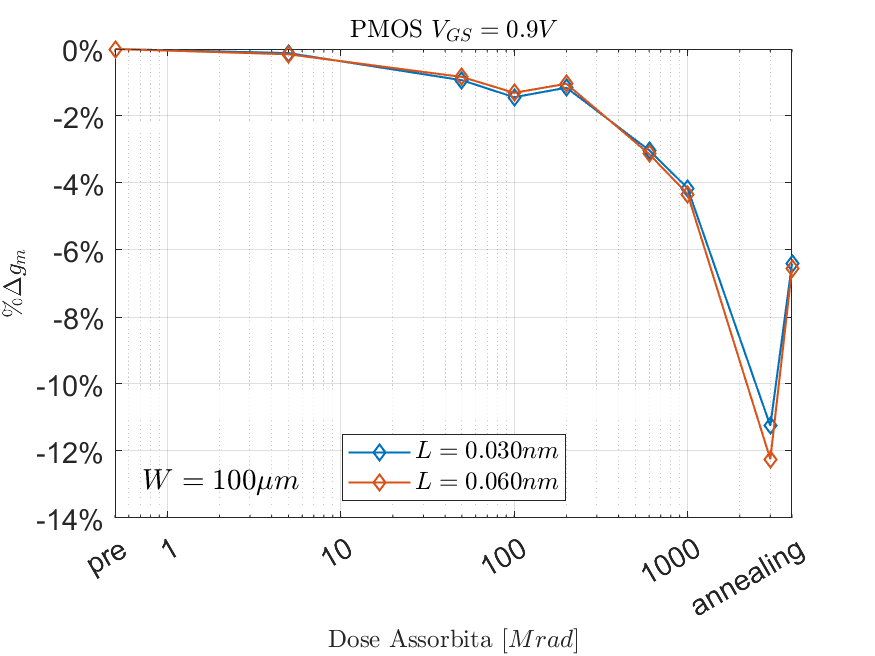
\includegraphics[width=0.49\textwidth]{./capitolo2/transconduttanza/delta_gm_P/vds_0_9/Delta_Gm_PMOS_Vds_0_9_W_100.png}

    \vspace{0.5cm}
    % W = 200
    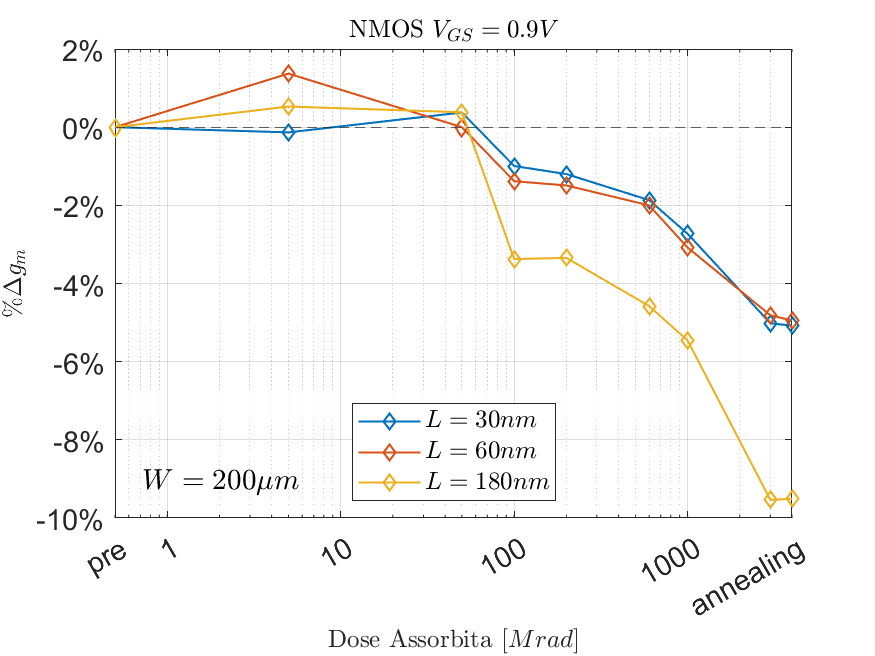
\includegraphics[width=0.49\textwidth]{./capitolo2/transconduttanza/delta_gm_N/vds_0_9/Delta_Gm_NMOS_Vds_0_9_W_200.png}
    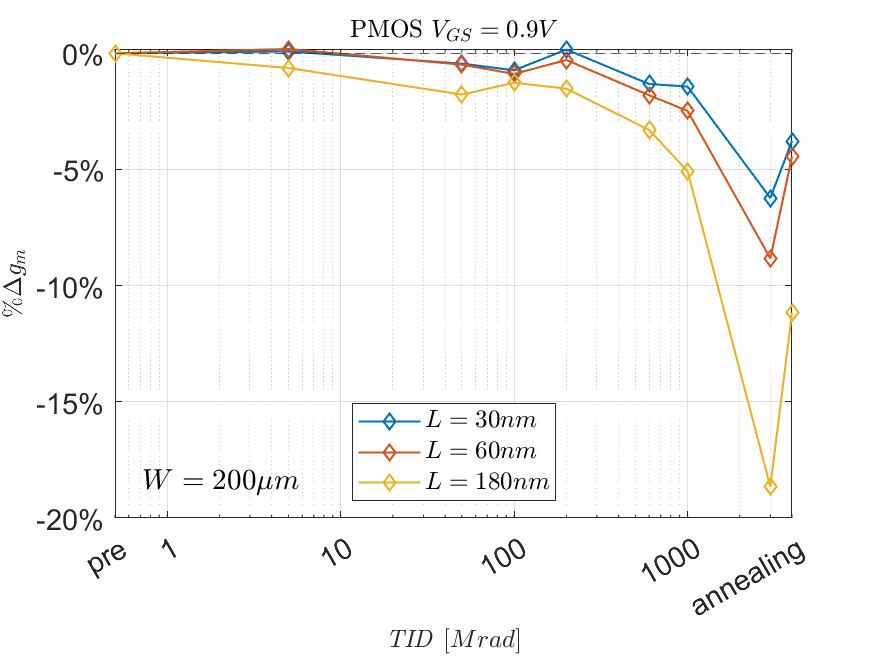
\includegraphics[width=0.49\textwidth]{./capitolo2/transconduttanza/delta_gm_P/vds_0_9/Delta_Gm_PMOS_Vds_0_9_W_200.png}
    % W = 600
    \vspace{0.5cm}

    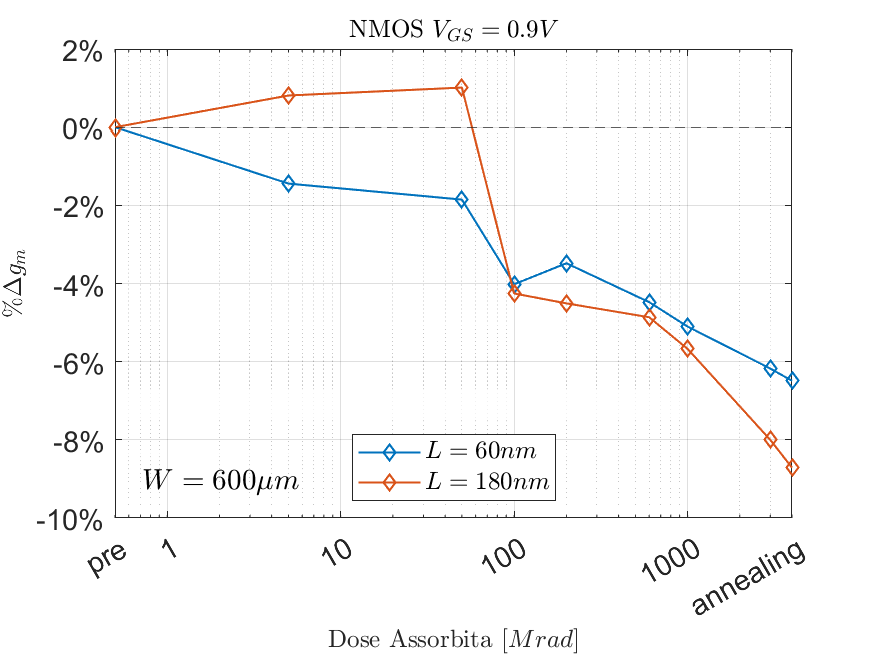
\includegraphics[width=0.49\textwidth]{./capitolo2/transconduttanza/delta_gm_N/vds_0_9/Delta_Gm_NMOS_Vds_0_9_W_600.png}
    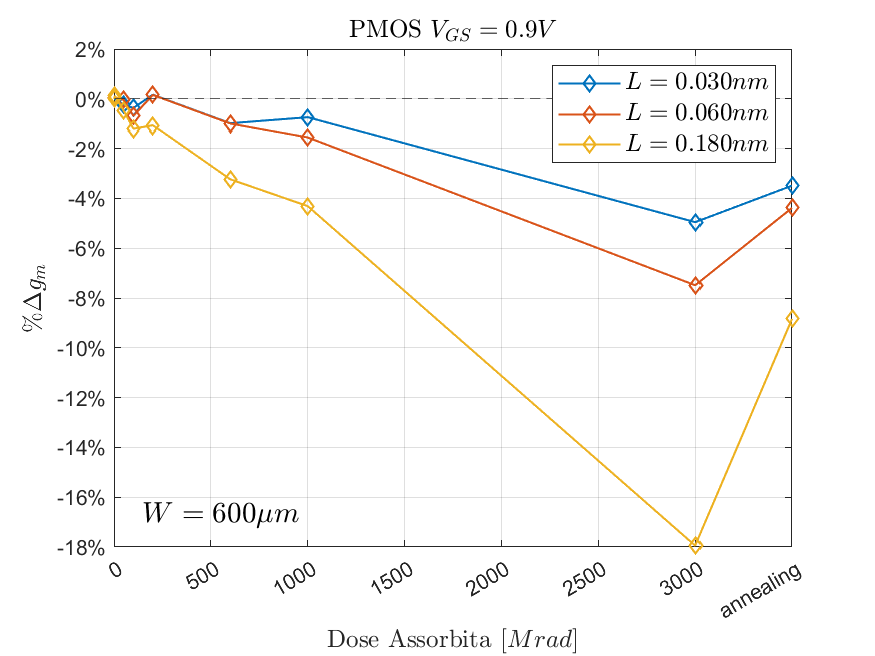
\includegraphics[width=0.49\textwidth]{./capitolo2/transconduttanza/delta_gm_P/vds_0_9/Delta_Gm_PMOS_Vds_0_9_W_600.png}
    \caption[Dati $\Delta g_m \%$ al variare della dose]{Curve $\Delta g_m $ percentuale al variare della dose assorbita: a sinistra i transistori MOSFET a canale N e a destra a canale P. I grafici sono raggruppati per larghezza di canale.}
    \label{fig:delta_gm}


\end{figure}